\section{Graphical function plotter}

The graphical function plotter is designed to take any of the implemented functions as input. This is obtained by creating an abstract \texttt{Function} super class, containing an \texttt{evaluate} method:

\begin{lstlisting}
public abstract double evaluate(double x);
\end{lstlisting}

By keeping the method abstract, each class extending the \texttt{Function} class must implement the method that evaluates the function for the argument \texttt{x}, and returns the value. 

The \texttt{Function} class is kept abstract since it would not make sense to evaluate or plot an unspecified function.\\
\\
We implemented the following subclasses by extending the superclass \texttt{Function}:

\subsection{\texttt{SineFunction}}
This function is implemented using the \texttt{sin(double a)} method from the \texttt{Math} class. The evaluate method (inherited from \texttt{Function}) returns the following:

\begin{lstlisting}
return a * Math.sin(b*x);
\end{lstlisting}

corresponding to the sine function $a \cdot \sin(b \cdot x)$, i.e. a sine wave with amplitude $a$, angular frequency $b$, and no phase shift. The requested example is shown in figure \ref{fig:f1}.

\begin{figure}[H]
    \begin{subfigure}{0.5\textwidth}
        \centering
    \includegraphics[width=0.7\linewidth]{GraphicalFunctionPlotter/fig/f1.png} 
    \caption{$f(x)=0.8\cdot \sin(2.1\cdot x)$.}
    \label{fig:f1}
    \end{subfigure}
    \begin{subfigure}{0.5\textwidth}
        \centering
    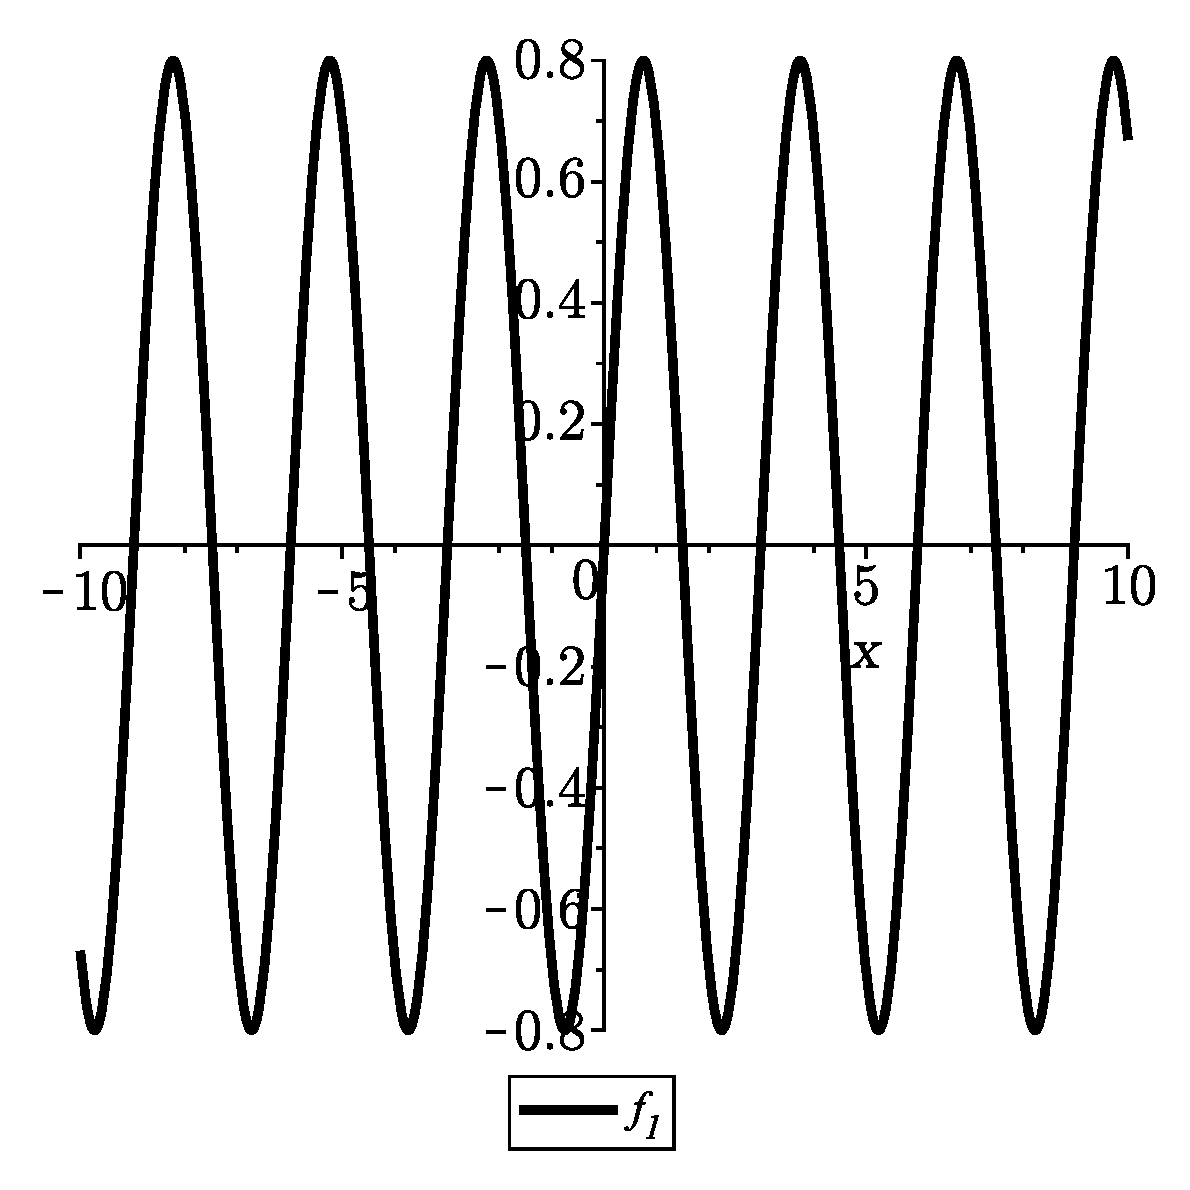
\includegraphics[width=0.7\linewidth]{GraphicalFunctionPlotter/fig/f1Check.eps}
    \caption{Same function plotted in Maple.}
    \label{fig:f1Check}
    \end{subfigure}
    \caption{Examples of the sine functions.}
\end{figure}
\newpage
\subsection{\texttt{PowerFunction}}
This function is implemented using the \texttt{pow(double a, double b)} method from the \texttt{Math} class. The \texttt{evaluate} method returns the following: 

\begin{lstlisting}
return b*Math.pow(Math.abs(x),a);
\end{lstlisting}

corresponding to the power function $b \cdot |x|^{a}$. The requested example is shown in figure \ref{fig:f2}. 


\begin{figure}[H]
    \begin{subfigure}{0.5\textwidth}
    \centering
    \includegraphics[width=0.7\linewidth]{GraphicalFunctionPlotter/fig/f2.png} 
    \caption{$f(x) = 2.1\cdot |x|^{2.0}$.}
    \label{fig:f2}
    \end{subfigure}
    \begin{subfigure}{0.5\textwidth}
    \centering
    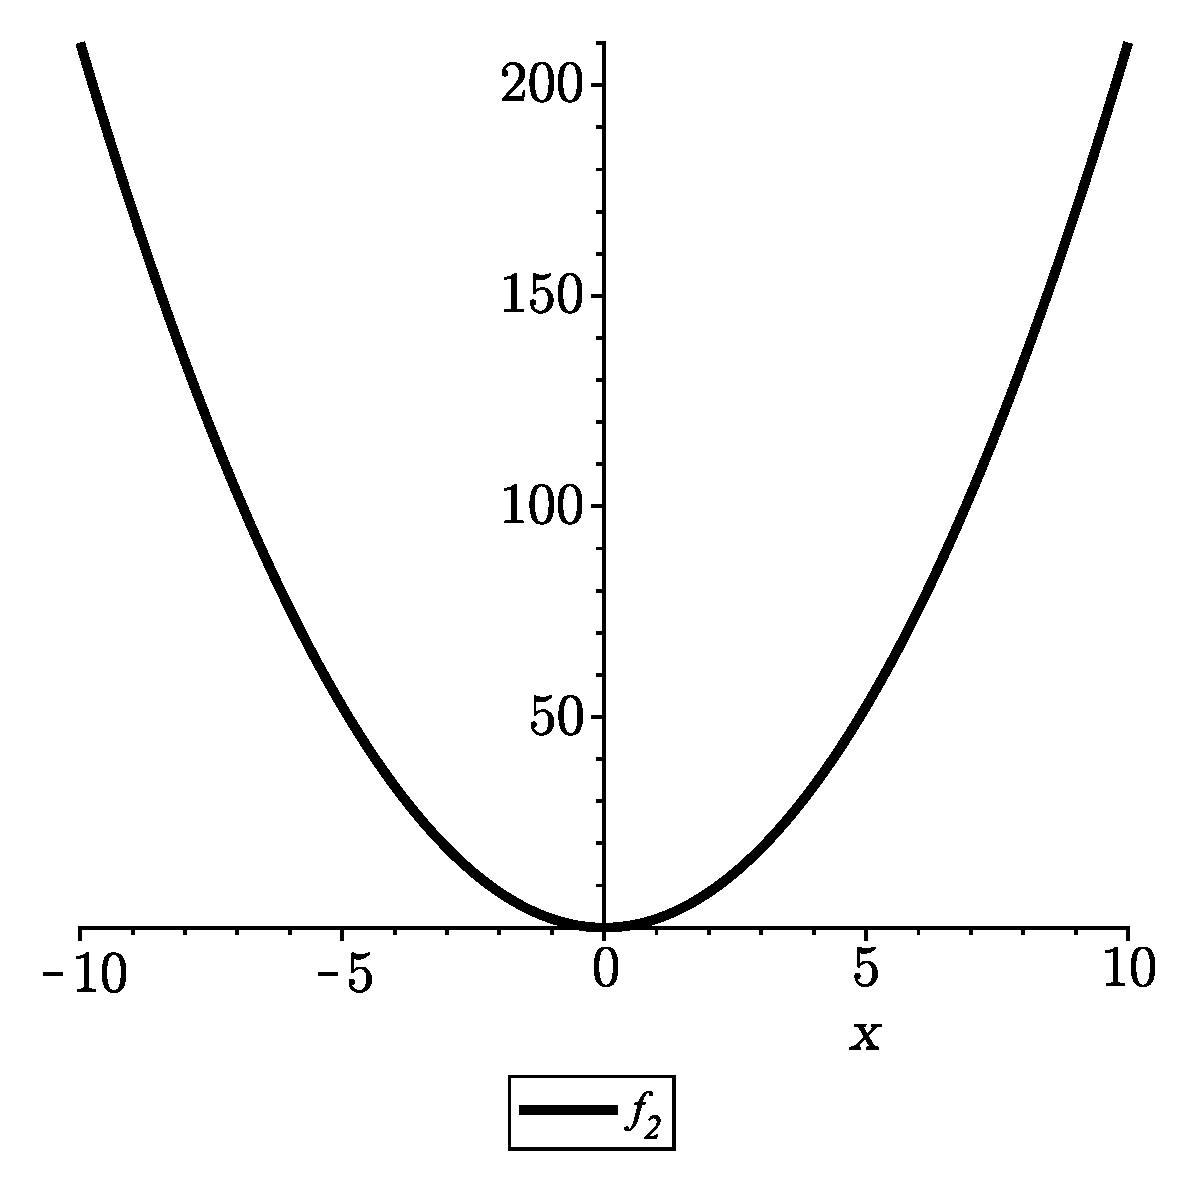
\includegraphics[width=0.7\linewidth]{GraphicalFunctionPlotter/fig/f2Check.eps}
    \caption{Same function plotted in Maple.}
    \label{fig:f2Check}
    \end{subfigure}
    \caption{Examples of the power functions.}
\end{figure}

\subsection{\texttt{ExponentialFunction}}
This function is also implemented using the \texttt{pow(double a, double b)} method from the \texttt{Math} class, as well as the built-in value of the constant e. The \texttt{evaluate} method returns the following:

\begin{lstlisting}
return a*Math.pow(Math.E,b*x);
\end{lstlisting}

corresponding to the exponential function $a \cdot \text{e}^{b \cdot x}$. \\
The requested example is shown in figure \ref{fig:f3}.

\begin{figure}[H]
    \begin{subfigure}{0.5\textwidth}
        \centering
        \includegraphics[width=0.7\linewidth]{GraphicalFunctionPlotter/fig/f3.png} 
        \caption{$f(x) = 3.2 \cdot \text{e}^{1.3 \cdot x}$.}
        \label{fig:f3}
    \end{subfigure}
    \begin{subfigure}{0.5\textwidth}
        \centering
        \includegraphics[width=0.7\linewidth]{GraphicalFunctionPlotter/fig/f3Check.eps}
        \caption{Same function plotted in Maple.}
        \label{fig:f3Check}
    \end{subfigure}
    \caption{Examples of the exponential functions.}
\end{figure}


\subsection{\texttt{PolynomialFunction}}
This function is also implemented using the \texttt{pow(double a, double b)} method from the \texttt{Math} class. The \texttt{evaluate} method returns the following:

\begin{lstlisting}
double sum = 0;
for(int i = 0; i < a.length; i++){
	sum += a[i]*Math.pow(x, i);
}
return sum;
\end{lstlisting}

Evaluating each value $a_n \cdot x^n$, returning the sum. \\
The requested examples are shown in figures \ref{fig:f4} and \ref{fig:f5}.

\begin{figure}[H]
    \begin{subfigure}{0.5\textwidth}
        \centering 
        \includegraphics[width=0.7\linewidth]{GraphicalFunctionPlotter/fig/f4} 
        \caption{$f(x)=0.4x^3-2.1x^2+4.1x-3.1$.}
        \label{fig:f4}
    \end{subfigure}
    \begin{subfigure}{0.5\textwidth}
        \centering
        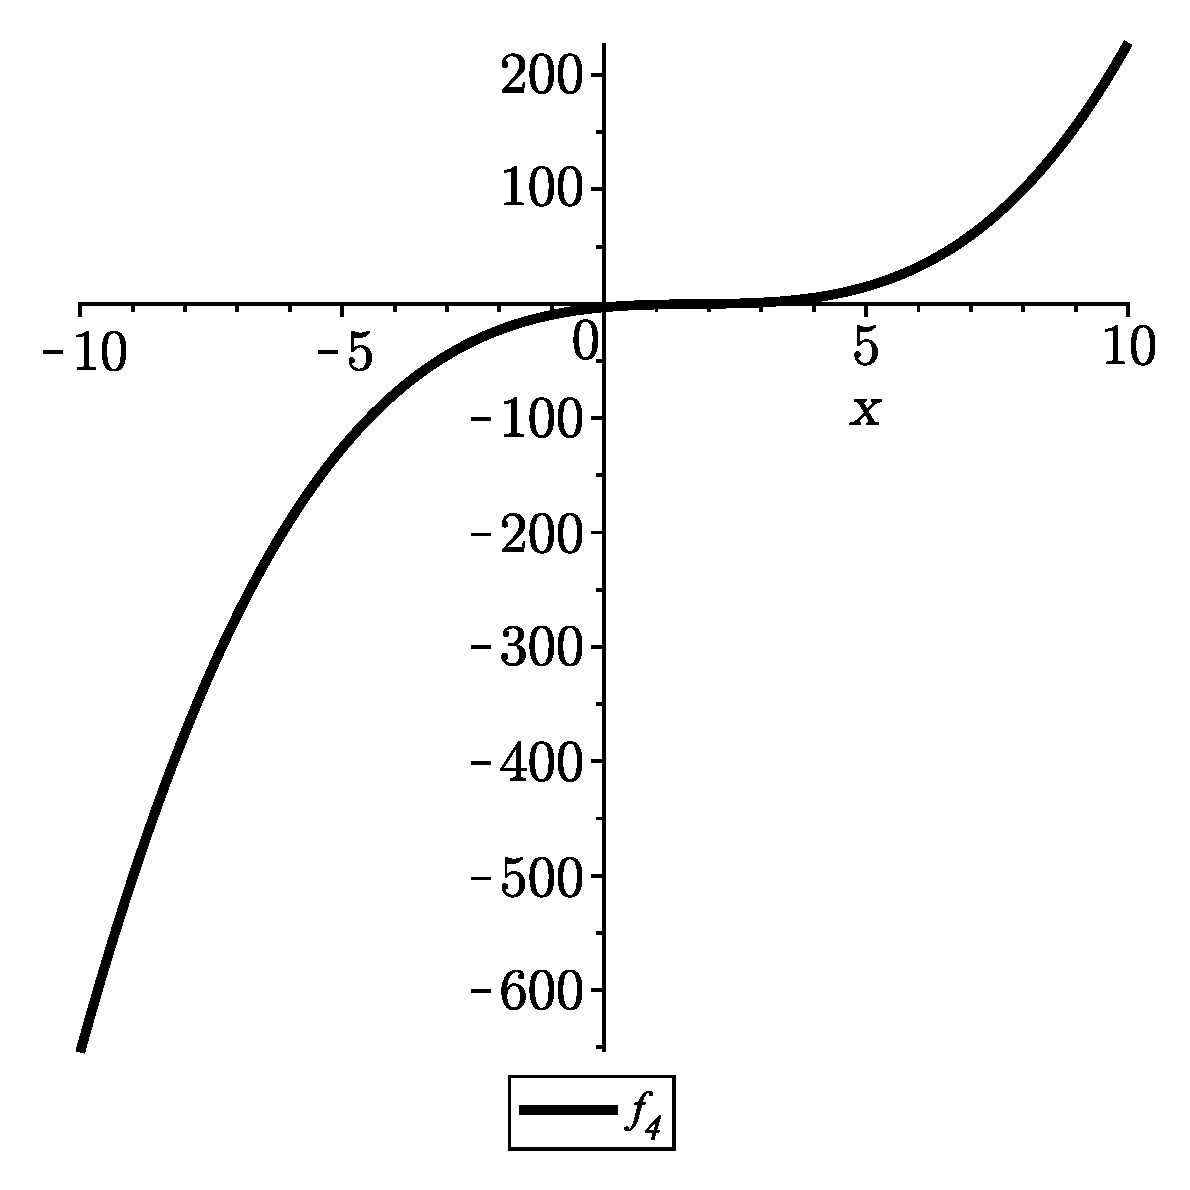
\includegraphics[width=0.7\linewidth]{GraphicalFunctionPlotter/fig/f4Check}
        \caption{Same function as \ref{fig:f4} plotted in Maple.}
        \label{fig:f4Check}
    \end{subfigure}
    \begin{subfigure}{0.5\textwidth}
        \centering
        \includegraphics[width=0.7\linewidth]{GraphicalFunctionPlotter/fig/f5}
        \caption{Taylor expansion of a sine function, 19 degrees.}
        \label{fig:f5}
    \end{subfigure}
    \begin{subfigure}{0.5\textwidth}
        \centering
        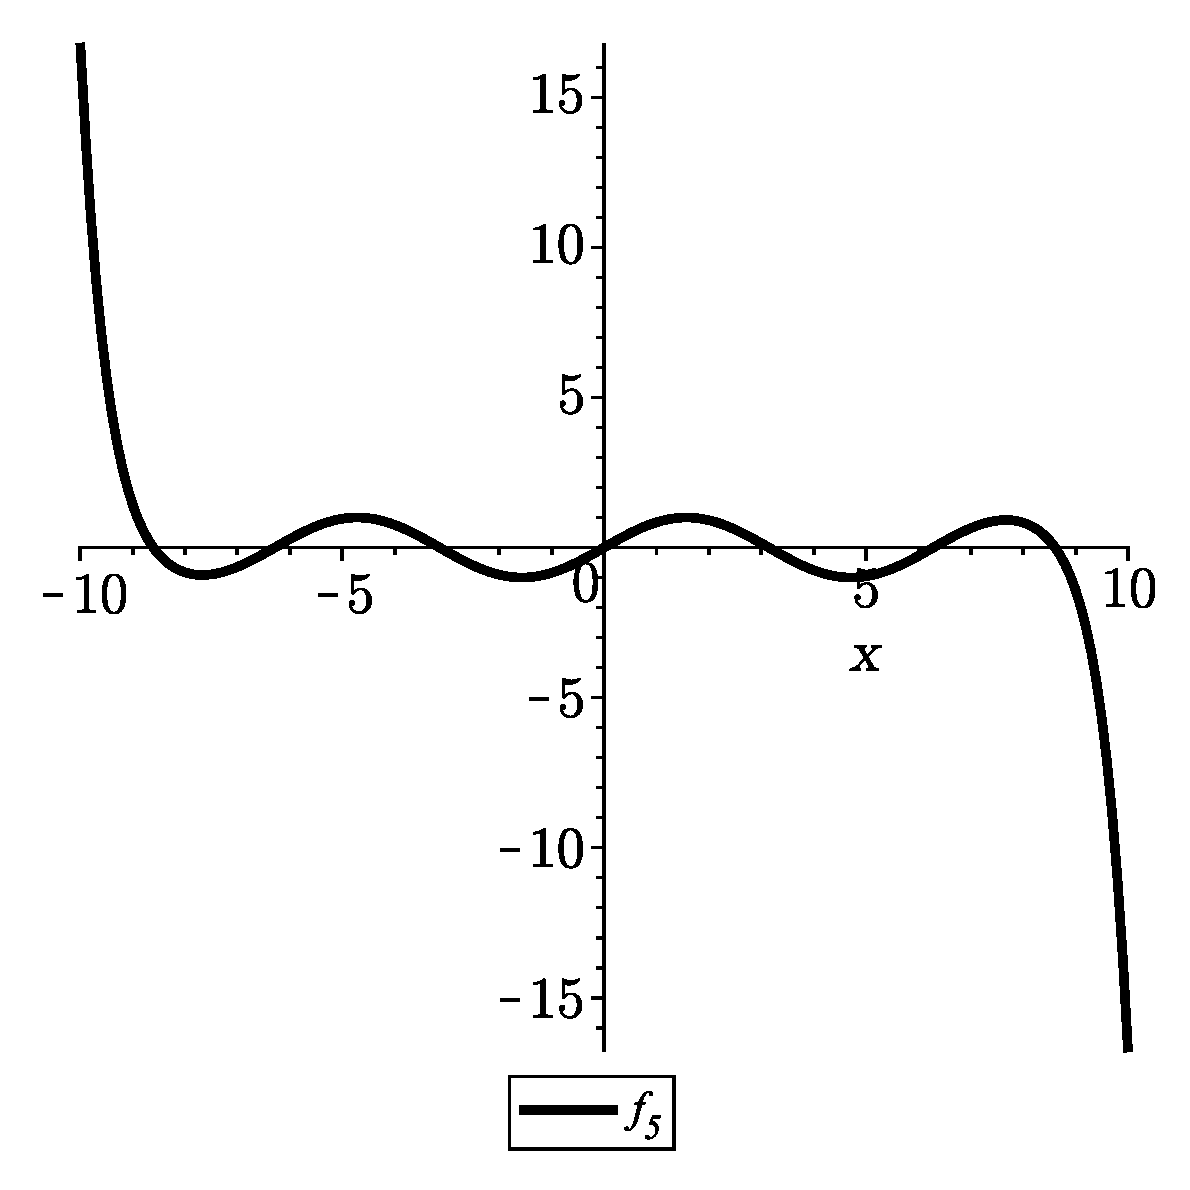
\includegraphics[width=0.7\linewidth]{GraphicalFunctionPlotter/fig/f5Check}
        \caption{Same function as \ref{fig:f5} plotted in Maple.}
        \label{fig:f5Check}
    \end{subfigure}
    \caption{Examples of the PolynomialFunction.}
 \end{figure}


\subsection{\texttt{SumFunction}}
This object takes an array of subclasses of the \texttt{Function} class as parameter. Each subclass in the array then calls its respective \texttt{evaluate} method, and their returned value is added to a running sum. This sum is then returned.

\begin{lstlisting}
double sum = 0;
for(int i = 0; i < f.length; i++){
	sum += f[i].evaluate(x);
}	
return sum;
\end{lstlisting}

If one of these subclasses correspond to a function with large function values, its return values may dominate the sum. Hence the plot may resemble just this particular function. E.g. if we sum a sine wave with values in the interval [$-2.1, \, 2.1$], some other "small-valued" functions, and an exponential function that diverges quickly, the plot may just look like the exponential. This effect is seen on the requested example on figure \ref{fig:f6}.


\begin{figure}[H]
    \begin{subfigure}{0.5\textwidth}
        \centering
        \includegraphics[width=0.7\linewidth]{GraphicalFunctionPlotter/fig/f6.png} 
        \caption{Sum of all previous functions.}
        \label{fig:f6}
    \end{subfigure}
    \begin{subfigure}{0.5\textwidth}
        \centering
        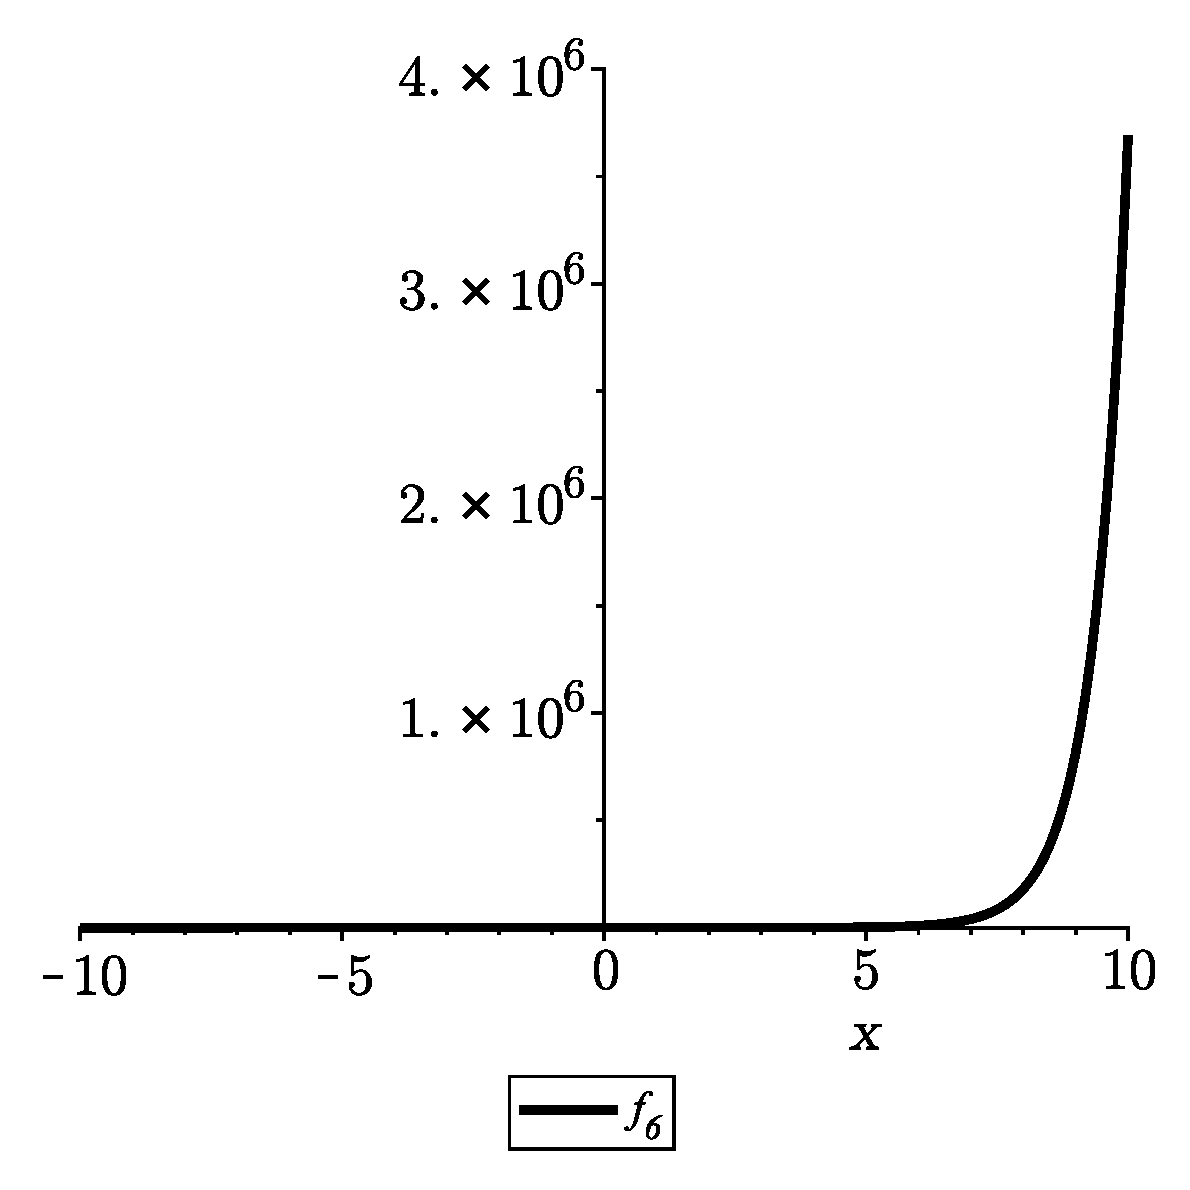
\includegraphics[width=0.7\linewidth]{GraphicalFunctionPlotter/fig/f6Check.eps}
        \caption{Same function plotted in Maple.}
        \label{fig:f6Check}
    \end{subfigure}
    \caption{Examples of the sum functions.}
\end{figure}

\subsection{\texttt{FunctionComposition}}
This object is also given an array of functions as argument. 
When running its \texttt{evaluate} method, it triggers a cascade of method calls using a method called \texttt{value}.

The \texttt{evaluate} method is implemented as follows:

\begin{lstlisting}
public double evaluate(double x) {
	return value(x, 0);
}

private double value(double x, int i){
	if(i >= f.length){
		return x;
	} else {
		return f[i].evaluate(value(x, i+1));
	}
}
\end{lstlisting}

As shown, a recursive method uses \texttt{value}, which creates a stack of functions only collapsing when the base-case is met. In this case, the base-case is, when all functions are put on the stack and \texttt{value} returns x. Each function is then evaluated in the output of the function above it (from the stack perspective), returning the final result through the \texttt{evaluate} method. The requested example is shown in figure \ref{fig:f7}.


\begin{figure}[H]
    \begin{subfigure}{0.5\textwidth}
        \centering
        \includegraphics[width=0.7\linewidth]{GraphicalFunctionPlotter/fig/f7.png} 
        \caption{$f_4(f_1(f_3(f_5(f_2(x)))))$.}
        \label{fig:f7}
    \end{subfigure}
    \begin{subfigure}{0.5\textwidth}
        \centering
        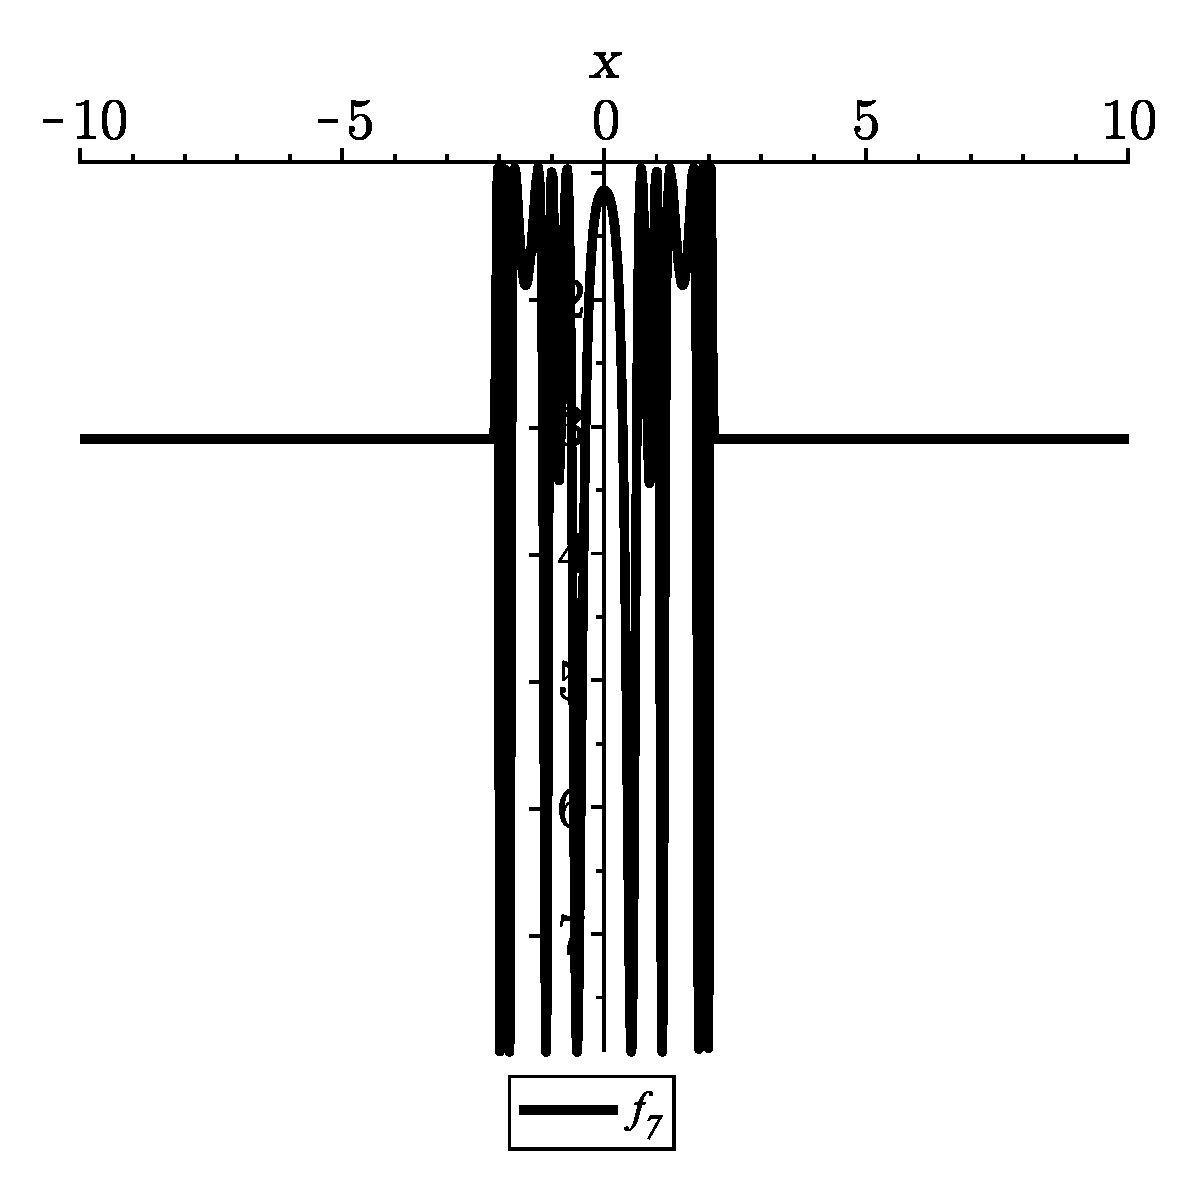
\includegraphics[width=0.7\linewidth]{GraphicalFunctionPlotter/fig/f7Check.eps}
        \caption{Same function plotted in Maple.}
        \label{fig:f7Check}
    \end{subfigure}
    \caption{Example of the composition function.}
\end{figure}

The \texttt{FunctionComposition} class is checked with several combinations of different functions as argument. In most cases, the implemented class and Maple return the same graphs, and hence outputs.\\
\\
However: some combinations of functions do not return the same graphs. We have noticed that these differences occur when power functions and especially exponential functions are compounded. We reckon that the problem is an overflow or precision error when calculating extreme numbers. An example of discrepancy is shown in figure \ref{fig:disc}.

\begin{figure}[H]
    \begin{subfigure}{0.5\textwidth}
        \centering
        \includegraphics[width=0.7\linewidth]{GraphicalFunctionPlotter/fig/f7Crude.png} 
        \caption{$f_4(f_1(f_3(f_5(f_2(x)))))$. With x from -2 to 2.}
        \label{fig:f7Crude}
    \end{subfigure}
    \begin{subfigure}{0.5\textwidth}
        \centering
        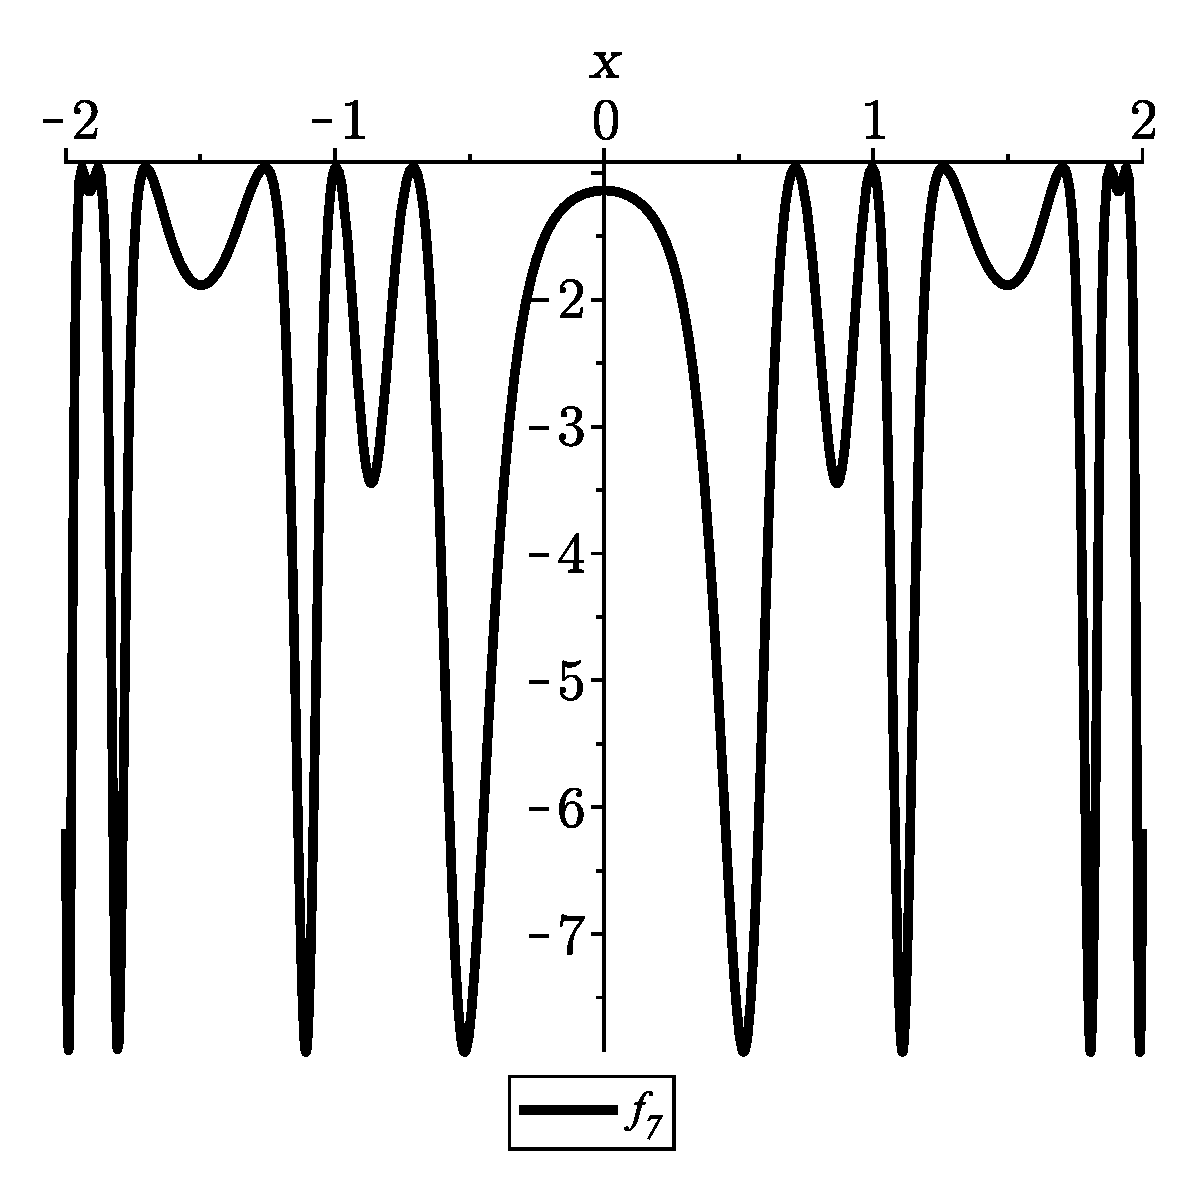
\includegraphics[width=0.7\linewidth]{GraphicalFunctionPlotter/fig/f7CheckCrude.eps}
        \caption{Same function plotted in Maple.}
        \label{fig:f7CheckCrude}
    \end{subfigure}
    \caption{The same function as figure \ref{fig:f7} with a shorter interval.}
    \label{fig:disc}
\end{figure}